\section{Theory}
	\subsection{P-N Junction Diode}
		A diode is any device that permits current to flow in just one direction. As a result, it functions as a variable resistor. A p-n junction is formed by joining two semiconductor materials, a p-type and an n-type. A p-type semiconductor is created by doping a semiconductor material (for example, Silicon) with a Group 13 acceptor material, which results in the generation of holes since the acceptor atom has one electron fewer in the valence shell to allow pairing with the electron of Si. Similarly, a Group 15 element is utilised in doping in an n-type semiconductor, resulting in an excess of electrons in the material, as seen in \hyperref[fig:1]{Figure 1}.

		\begin{figure}[h]
			\centering
			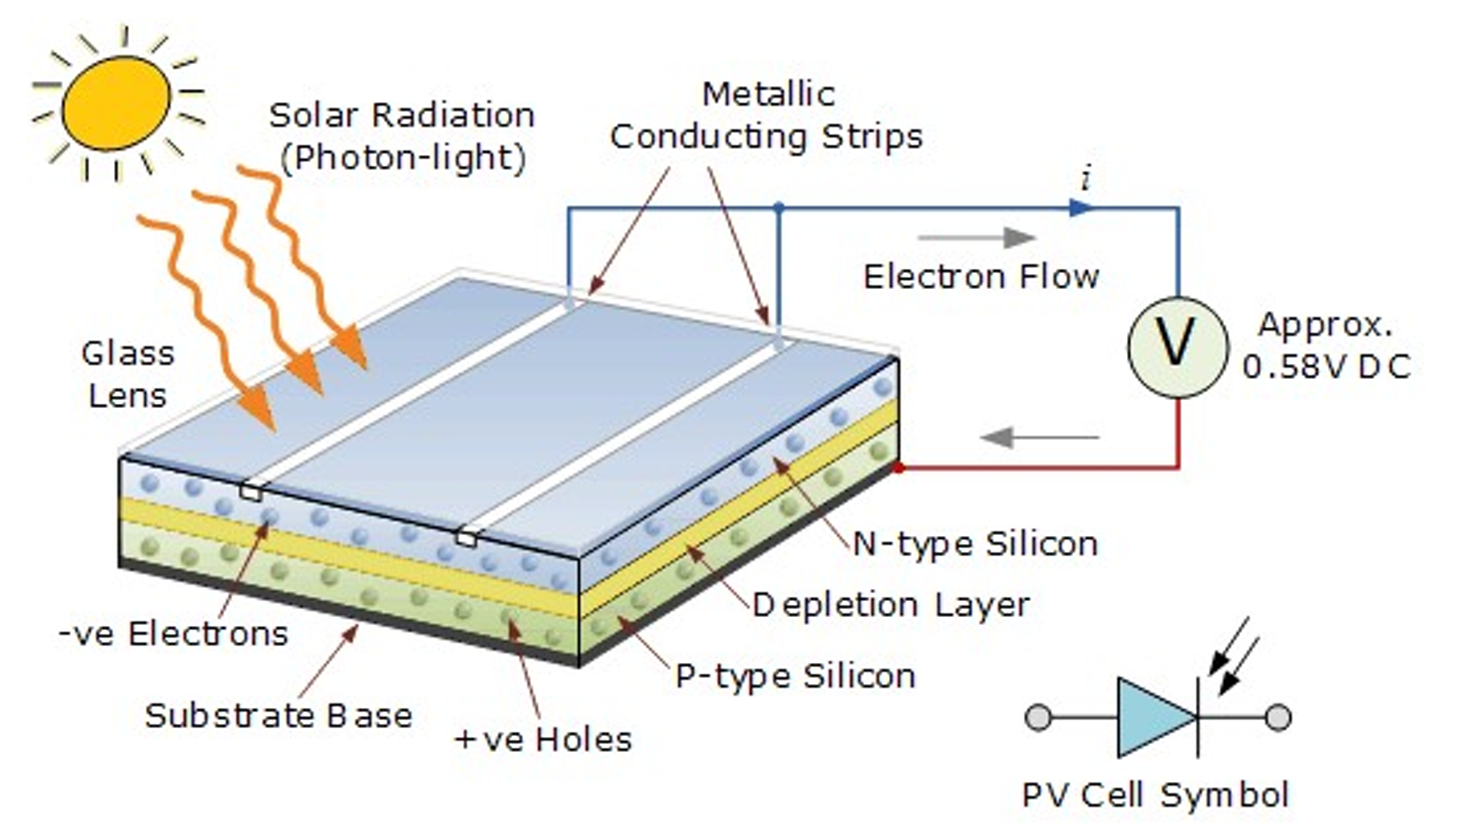
\includegraphics[width=0.8\columnwidth]{images/theory1.png}
			\caption{Construction of Solar Cell}
			\label{fig:1}
		\end{figure}
		
		Surplus electrons from the n side and excess holes from the p side migrate towards the junction to recombine when the two types of materials are combined (more stable state). When they join at the junction, they leave positively charged ions on the n side and negatively charged ions on the p side behind. When the electric field formed by the charged ions balances the diffusion of electron hole pairs, it becomes saturated. As a result, in the state, a depletion area forms at the diode junction, with a junction potential that prohibits further passage of electrons and holes. There are still motions such as drift current when, as a result of collisions, certain electrons and holes (e-h) on the n and p sides may obtain enough kinetic energy to overcome the potential barrier. When e-h couples develop within the depletion area, the diffusion current is cancelled out by the drift current, which is swiftly dragged towards the n and p sides by the electric field on the ions. This drift current becomes noticeable in a solar cell.

	\subsection{Solar Cell}

		A solar cell, also known as a photovoltaic cell, is a form of active transducer and the fundamental unit of a solar energy generation system that converts light energy directly into electrical energy. It is essentially a semiconductor p-n junction diode that generates charge carriers (e-h pair) by absorbing energy from falling radiation. When sunlight strikes a solar cell, photons with energies larger than the band gap of the semiconductor are absorbed by the cell, resulting in the formation of an electron-hole (e-h) pair. When these e-h pairs develop in the deplection zone, they migrate to the n- and p- sides of the p-n junction as drift current due to the electrostatic force of the field across the junction. As more radiation is absorbed, charges accumulate on the two sides of the cell, resulting in a potential difference. A solar or photovoltaic cell typically features a negative front contact and a positive rear contact. When connected to the terminals of a battery, the charge carriers begin to flow, producing current. At ambient temperature, the band gap for silicon is $E_g = 1.1eV$, and the diffusion potential is $U_D = 0.5$ to $0.7V$.

	\subsection{I-V Characteristics}

		Solar Cell I-V Characteristics Curve is the superposition of the I-V curves of the solar cell diode in absence (dark) and in presence of light. The connection is made in reverse bias, and depending on the load of the circuit, we get different values. Solar Cell I-V Characteristics Curve is the superposition of the I-V curves of the solar cell diode in absence (dark) and in presence of light. Illuminating a cell adds to the normal ”dark” currents in the diode so that the diode law for q electronic charge, n ideality factor and at T temperature becomes:

		\begin{equation}
			\label{eq:1}
			I(V) = I_0\left[e^{\frac{qV}{nKT}}-1\right] - I_L
		\end{equation}
		
		where $I_0$ is the diode leakage current in absence of light and $I_L$ is the current generated by light. A typical circuit for measuring I-V characteristics is shown in the \hyperref[fig:2]{Figure 2}.

		\begin{figure}[h]
			\centering
			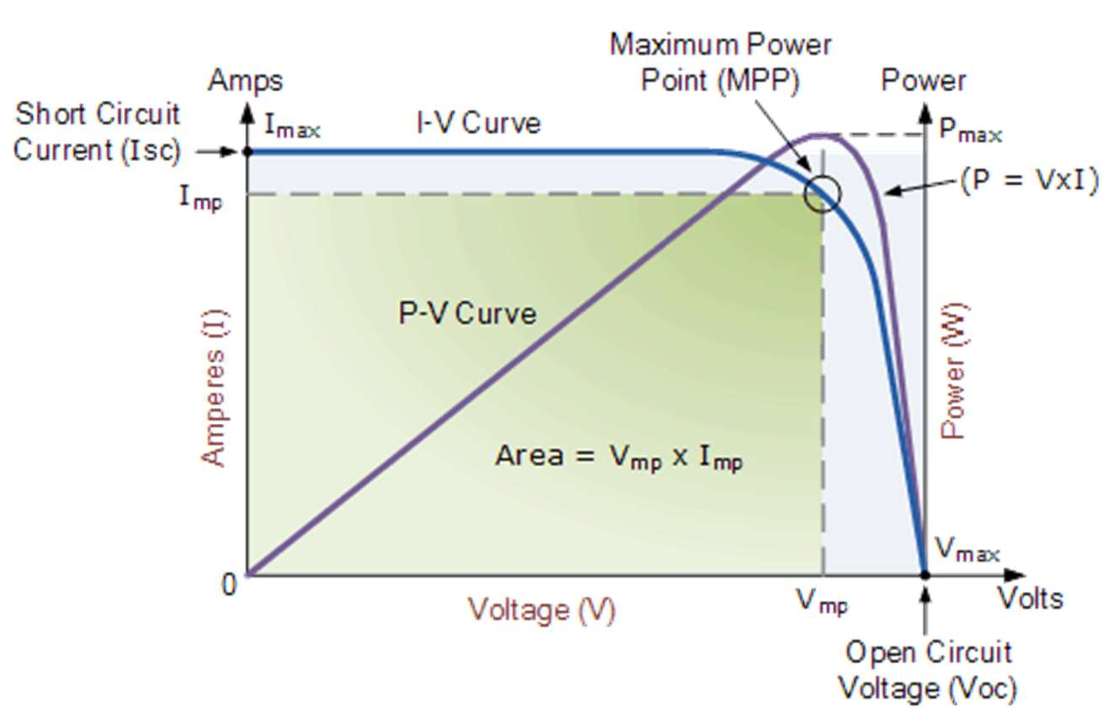
\includegraphics[width=0.8\columnwidth]{images/theory2.png}
			\caption{I-V curve and power curve of a typical solar cell}
			\label{fig:2}
		\end{figure}

		Due to comparable characteristics, the curve approaches the forward bias I-V curve of an inverted diode. The solar cell's many properties may be calculated from these features. These factors determine a solar panel's rating:

		\begin{enumerate}
			\item \textbf{Short-circuit current (ISC):} the flow of electricity through a solar cell when it is shorted out. The voltage across the solar cell is 0 since there are no charge carriers that have accumulated in the event of a short circuit. Therefore, the highest current that may be extracted from a solar cell is the shortcircuit current.
			\item \textbf{Open-circuit voltage (VOC):} At zero current, it is the greatest voltage a solar cell is capable of producing. When the circuit is open, something happens. The solar cell's forward bias, which results from the junction's bias with the light-generated current, is represented by the open-circuit voltage.
			\item \textbf{Maximum power point (MPP):} Maximum power, which occurs when the tangency of the curve is $-1$ and is designated as the MPP in the picture, is a visual representation of the `squareness' of the solar cell. It is also the size of the biggest rectangle that will fit in the I-V curve.
			\item \textbf{Fill Factor (FF):} The FF is defined as the ratio of the maximum power from the solar cell to the product of VOC and ISC.
			\item \textbf{Efficiency:} It determines the performance of one solar cell to another and is defined as the ratio of energy output from the solar cell to input energy from the sun.
		\end{enumerate}

	\subsection{Direct and Indirect Band Gap}

		The lowest energy difference between the top of the valence band and the bottom of the conduction band determines the band gap. However, the top of the valence band and the bottom of the conduction band might not be at the same electron momentum value in the momentum space. If so, it is referred to as an indirect band gap. A straight band gap is what is known when the conduction minima and value maxima occur at the same value of the electron momentum, as seen in the \hyperref[fig:3]{Figure 3}.

		\begin{figure}[h]
			\centering
			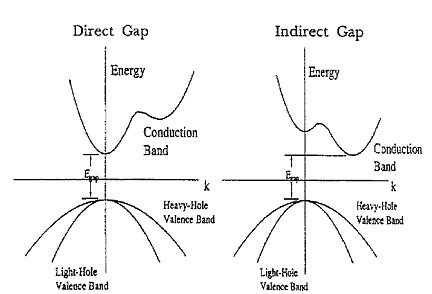
\includegraphics[width=0.8\columnwidth]{images/theory3.jpeg}
			\caption{Direct and Indirect Band Gap}
			\label{fig:3}
		\end{figure}

		When it comes to a direct band gap semiconductor, generating an electron-hole pair by a photon with energy E is relatively easy because the electron does not need to have much momentum. Conversely, creating an e-h pair in the indirect band gap takes more time as a photon has to alter the momentum. To gain or lose momentum, the electron must interact with both the photon and a phonon, a lattice vibration.
		
		As a result, e-h pairs created indirectly have longer lifetimes compared to those generated directly. For solar cells, we require high e-h pair lifetimes to enable their movement and buildup on the diode's sides. Hence, we make use of indirect band gap semiconductors like silicon. Conversely, we utilize direct gap materials like gallium arsenide in creating optical devices such as LEDs and semiconductor lasers, as the photodiode effect mandates the excited electron to rapidly de-excite and discharge radiation

	\subsection{Experimental Setup}

	The circuit schematic below in \hyperref[fig:4]{Figure 4} shows the experimental setup. A potentiometer is used to modulate resistance in the circuit, and a multimeter is used to measure current. The solar cell is put in a well-lit area. For the purpose of measuring the voltage across the cell, a second multimeter is connected in parallel. To cover the solar cell and tabulate the values of I and V for various loads applied, we have several filters, including green, yellow, pink, and red.

	\begin{figure}[h]
		\centering
		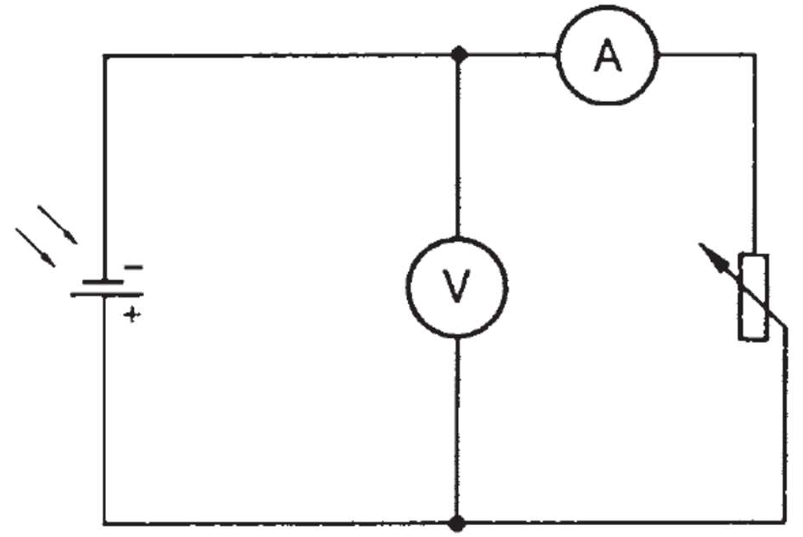
\includegraphics[width=0.8\columnwidth]{images/theory4.png}
		\caption{Experimental Setup}
		\label{fig:4}
	\end{figure}
